\documentclass[12pt]{article}
% ----------------------------------------库函数⬇️
\usepackage[a4paper,left=25mm,right=25mm,top=25mm,bottom=25mm]{geometry}  
\usepackage{ctex}        % 中文库
\usepackage{titletoc}    % 目录库
\usepackage{fancyhdr}    % 页眉库
\usepackage{url}         % 链接库
\usepackage{graphicx}    % 图片库
\usepackage{float}       % 数学库
\usepackage{amsmath}     % 复杂数学库
\usepackage{amssymb}     % 花体字符库
\usepackage{algorithm}   % 算法流程图库
\usepackage{algorithmic} % 算法流程图库
\usepackage{listings}    % 代码块库
\usepackage{xcolor}      % 代码块颜色库
\usepackage{multirow}    % 多行合并表格库
\usepackage{array}       % 表格库
\usepackage{booktabs}    % 三线表库
% ----------------------------------------库函数⬆️
% ----------------------------------------正文内英文字体设置⬇️
\setmainfont{Times New Roman}
% ----------------------------------------正文内英文字体设置⬇⬆️
% ----------------------------------------代码风格设置⬇️
\lstset{
    basicstyle          =   \sffamily,          % 基本代码风格
    keywordstyle        =   \bfseries,          % 关键字风格
    commentstyle        =   \rmfamily\itshape,  % 注释的风格,斜体
    stringstyle         =   \ttfamily,          % 字符串风格
    flexiblecolumns,                            % 列间自由宽度
    numbers             =   left,               % 行号的位置在左边
    showspaces          =   false,              % 是否显示空格
    numberstyle         =   \zihao{-5}\ttfamily,% 行号的样式,小五号,tt等宽字体
    showstringspaces    =   false,              % 显示空格
    captionpos          =   t,                  % 这段代码的名字所呈现的位置,t指的是top上面
    frame               =   lrtb,               % 显示边框
}
\lstdefinestyle{Python}{
    language        =   Python,                 % 语言选Python
    basicstyle      =   \zihao{-5}\ttfamily,
    numberstyle     =   \zihao{-5}\ttfamily,
    keywordstyle    =   \color{blue},
    keywordstyle    =   [2] \color{teal},
    stringstyle     =   \color{magenta},
    commentstyle    =   \color{red}\ttfamily,
    breaklines      =   true,                   % 自动换行
    columns         =   fixed,                  % 固定字间距
    basewidth       =   0.5em,
}
\lstdefinestyle{C++}{
    language        =   C++,                    % 语言选C++
    basicstyle      =   \zihao{-5}\ttfamily,
    numberstyle     =   \zihao{-5}\ttfamily,
    keywordstyle    =   \color{blue},
    keywordstyle    =   [2] \color{teal},
    stringstyle     =   \color{magenta},
    commentstyle    =   \color{red}\ttfamily,
    breaklines      =   true,                   
    columns         =   fixed,                  
    basewidth       =   0.5em,
}
% ----------------------------------------代码风格设置⬆️
% ----------------------------------------正文⬇️
\begin{document}
% 封面
\begin{titlepage}
	\center
    
\includegraphics[width=10cm]{UIR.png}\\[3cm]
    \begin{flushleft}
        \text{\zihao{3}\heiti\qquad\qquad 中文标题:在这里输入中文标题}\\[0.5cm] 
        \text{\zihao{3}\heiti\qquad\qquad 英文标题:Enter your title name here}\\[3cm] 
    \end{flushleft}
	\begin{minipage}{0.5\textwidth}
		\begin{flushleft}\zihao{3}
			\heiti 届\quad\quad\ \ \, 别:xxxx级\\[0.5cm]
			\heiti 院\quad\quad\ \ \, 系:网络空间安全学院\\[0.5cm]
            \heiti 专业与方向:网络空间安全\\[0.5cm]
            \heiti 姓\quad\quad\ \ \, 名:xxx\\[0.5cm]
            \heiti 学\quad\quad\ \ \, 号:xxxxxxxx\\[0.5cm]
            \heiti 指\;导\;\,教\;师:xxx
		\end{flushleft}
	\end{minipage}\\[3cm]
    \text{\zihao{3}\heiti 完成时间:20xx年x月}
	\vfill 
\end{titlepage}
% 行间距
\linespread{1.5}
% 页眉
\pagestyle{fancy}
\fancyhead[C]{文章题目}
\fancyhead[L, R]{}
% 标题
\pagenumbering{Roman}
\title{\songti \zihao{2} \textbf{题目}}
\author{\fangsong \zihao{-3}作者1 \quad 作者2}
\date{}
\maketitle
% 摘要
\ctexset{abstractname = {\zihao{-4}摘要}}
\begin{abstract}
    \zihao{-4}\fangsong 中文摘要\\
    \zihao{-4} \textbf{\heiti 关键字:}中文关键词1;中文关键词2
\end{abstract}
\ctexset{abstractname = {\zihao{-4}Abstract}}
\begin{abstract}
    \zihao{-4} 英文摘要 \\
    \zihao{-4} \textbf{\heiti Keywords:}英文关键词1;英文关键词2
\end{abstract}
% 目录
\newpage
\tableofcontents
\contentsmargin{0pt}
\renewcommand\contentspage{\thecontentspage}
\dottedcontents{section}[20pt]{\vspace{1mm}\bfseries\songti\zihao{-4}}{25pt}{5pt}
\dottedcontents{subsection}[50pt]{\vspace{1mm}\songti\zihao{-4}}{30pt}{5pt}
\dottedcontents{subsubsection}[80pt]{\vspace{1mm}\songti\zihao{-4}}{40pt}{5pt}
% 文章内容
\newpage
\pagenumbering{arabic}
\section{\songti\zihao{-4}第一部分}
\section{\songti\zihao{-4}第二部分}
\subsection{\songti\zihao{-4}第二部分第一小节}
\subsubsection{\songti\zihao{-4}第二部分第一小节第一分节}
\section{\songti\zihao{-4}第三部分}
% 简单公式
\clearpage
\songti\zihao{-4}在语句内添加公式用$a^2=b^2+c^2$来表示
\songti\zihao{-4}在语段间添加公式用$$a^2=b^2+c^2$$来表示
% 分点
\clearpage
\songti\zihao{-4}分点可以用以下代码表示:
\begin{enumerate}
    \songti\zihao{-4}\item xxx
    \songti\zihao{-4}\item xxx
    \songti\zihao{-4}\item xxx
\end{enumerate}
或
\begin{itemize}
    \songti\zihao{-4}\item xxx
    \songti\zihao{-4}\item xxx
    \songti\zihao{-4}\item xxx
\end{itemize}
% 图片
\clearpage
\songti\zihao{-4}展示图片可以用如图1来表示:
\begin{figure}[H]
    \label{fig:图片}
    \centering
    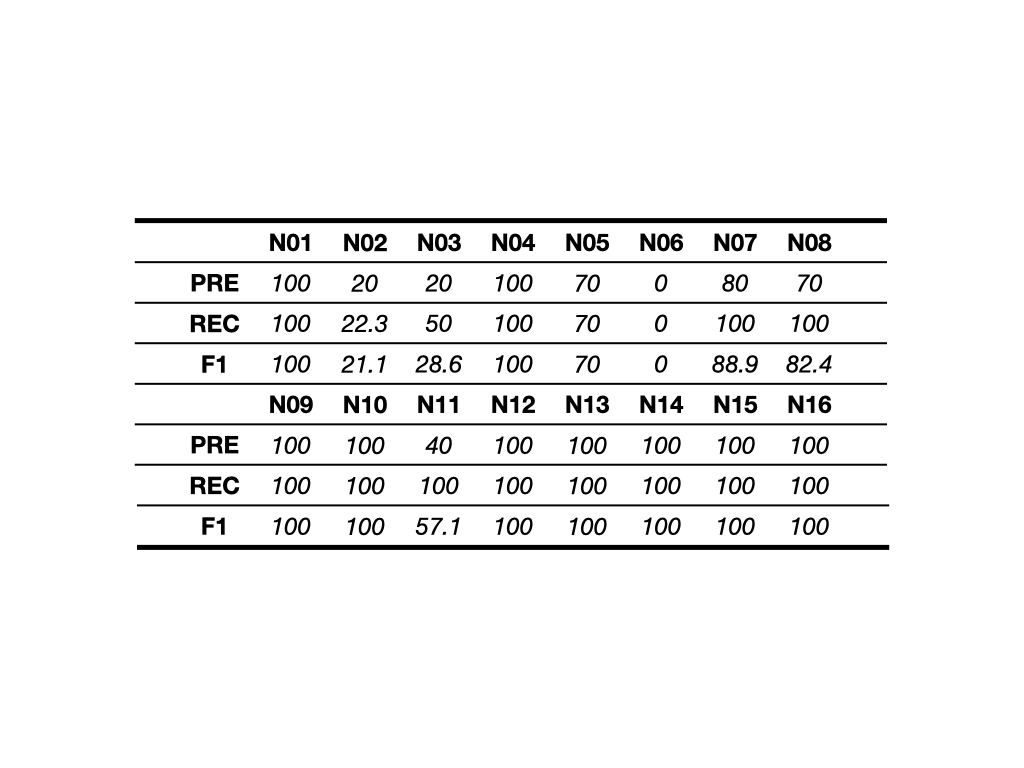
\includegraphics[scale=0.5,trim=150 220 150 220,clip]{图片.jpeg}
    \caption{\fangsong 这是一张图片}
\end{figure}
% 表格
\clearpage
\songti\zihao{-4}展示表格可以用如表1来表示:
\begin{table}[H]
    \centering
    \begin{tabular}{ccc}
        \hline
        Parameters & T & $k_1$ \\ 
        \hline
        Values & 0.02s & 10 \\ 
        \hline
    \end{tabular}
    \caption{\fangsong 这是一个表格}
\end{table}
% 伪代码
\clearpage
\songti\zihao{-4}展示算法/伪代码可以用下面的方法来表示:
\begin{algorithm}[htb]
    \caption{ Framework of ensemble learning for our system.}
    \label{alg:Framwork}
    \begin{algorithmic}[1] % 这个1表示每一行都显示数字
    \REQUIRE ~~\\ % 算法的输入参数:Input
        The set of positive samples for current batch, $P_n$;\\
        The set of unlabelled samples for current batch, $U_n$;\\
        Ensemble of classifiers on former batches, $E_{n-1}$;
    \ENSURE ~~\\ % 算法的输出:Output
        Ensemble of classifiers on the current batch, $E_n$;
        \STATE Extracting the set of reliable negative and/or positive samples $T_n$ from $U_n$ with help of $P_n$;
        \STATE Training ensemble of classifiers $E$ on $T_n \cup P_n$, with help of data in former batches;
        \STATE $E_n=E_{n-1}\cup E$;
        \STATE Classifying samples in $U_n-T_n$ by $E_n$;
        \STATE Deleting some weak classifiers in $E_n$ so as to keep the capacity of $E_n$;
    \RETURN $E_n$; % 算法的返回值
    \end{algorithmic}
\end{algorithm}
\begin{algorithm}
    \caption{An example}
    \label{alg:2}
    \begin{algorithmic}
        \STATE {set $r(t)=x(t)$}
        \REPEAT
        \STATE set $h(t)=r(t)$
        \REPEAT
        \STATE set $h(t)=r(t)$
        \UNTIL{B}
        \UNTIL{B}
    \end{algorithmic}
\end{algorithm}
\begin{algorithm}
    \caption{Calculate $y = x^n$}
    \label{alg:3}
    \begin{algorithmic}
        \REQUIRE $n \geq 0 \vee x \neq 0$
        \ENSURE $y = x^n$
        \STATE $y \Leftarrow 1$
    \IF{$n < 0$}
        \STATE $X \Leftarrow 1 / x$
        \STATE $N \Leftarrow -n$
    \ELSE
        \STATE $X \Leftarrow x$
        \STATE $N \Leftarrow n$
    \ENDIF
    \WHILE{$N \neq 0$}
        \IF{$N$ is even}
            \STATE $X \Leftarrow X \times X$
            \STATE $N \Leftarrow N / 2$
        \ELSE[$N$ is odd]
            \STATE $y \Leftarrow y \times X$
            \STATE $N \Leftarrow N - 1$
        \ENDIF
    \ENDWHILE
    \end{algorithmic}
\end{algorithm}
\begin{algorithm}[h]
    \caption{An example for format For \& While Loop in Algorithm}
    \label{alg:4}
    \begin{algorithmic}[1]
        \FOR{each $i \in [1,9]$}
            \STATE initialize a tree $T_{i}$ with only a leaf (the root);\
            \STATE $T=T \cup T_{i};$\
        \ENDFOR
        \FORALL {$c$ such that $c \in RecentMBatch(E_{n-1})$}
            \STATE $T=T \cup PosSample(c)$;
        \ENDFOR
        \FOR{$i=1$; $i<n$; $i++$ }
            \STATE $//$ Your source here;
        \ENDFOR
        \FOR{$i=1$ to $n$}
            \STATE $//$ Your source here;
        \ENDFOR
            \STATE $//$ Reusing recent base classifiers.
        \WHILE {$(|E_n| \leq L_1 )and( D \neq \phi)$}
            \STATE Selecting the most recent classifier $c_i$ from $D$;
            \STATE $D=D-c_i$;
            \STATE $E_n=E_n+c_i$;
        \ENDWHILE
    \end{algorithmic}
\end{algorithm}
% 复杂公式
\clearpage
\songti\zihao{-4}展示复杂公式可以用下面的方法来表示:
\begin{gather}    % 会产生编号
	a+b=b+a\\
	ab=ba
\end{gather}
\begin{gather*}    % 不会产生编号
a \times b=b \times a\\
ab=ba   
\end{gather*}
\begin{gather}    % 会编号
a+b=b+a \notag \\    % \notag阻止编号
ab=ba   \notag     % \notag阻止编号
\end{gather}
\begin{align}
	x &= t + \cos t + 1\\
	y &= 2\sin t
\end{align}
\begin{equation}
	\begin{split}
	\cos 2x &= \cos^2 x - \sin^2 x\\
	&= 2\cos^2 x - 1
	\end{split}
\end{equation}
\begin{equation}
	D(x) = \begin{cases}
	1, &\text{如果} x \in \mathbb{Q}\\    % mathbb花体字符
	0, &\text{如果} x \in \mathbb{R}\setminus\mathbb{Q}	
		   \end{cases}    % \text是为了在数学公式中处理中文
\end{equation}
% 代码块
\clearpage
\songti\zihao{-4}展示代码块可以用下面的方法来表示:
\lstinputlisting[
    style       =   Python,
    caption     =   {\bf test.py},
    label       =   {test.py}
]{test.py}
\lstinputlisting[
    style       =   C++,
    caption     =   {\bf test.cpp},
    label       =   {test.cpp}
]{test.cpp}
% 参考引用
\clearpage
\songti\zihao{-4}参考文献这样使用\cite{ref2}
\begin{thebibliography}{99}  
    \bibitem{ref1}Zheng L, Wang S, Tian L, et al., Query-adaptive late fusion for image search and person re-identification, Proceedings of the IEEE Conference on Computer Vision and Pattern Recognition, 2015: 1741-1750.  
    \bibitem{ref2}Arandjelović R, Zisserman A, Three things everyone should know to improve object retrieval, Computer Vision and Pattern Recognition (CVPR), 2012 IEEE Conference on, IEEE, 2012: 2911-2918.  
    \bibitem{ref3}Lowe D G. Distinctive image features from scale-invariant keypoints, International journal of computer vision, 2004, 60(2): 91-110.  
    \bibitem{ref4}Philbin J, Chum O, Isard M, et al. Lost in quantization: Improving particular object retrieval in large scale image databases, Computer Vision and Pattern Recognition, 2008. CVPR 2008, IEEE Conference on, IEEE, 2008: 1-8.  
\end{thebibliography}
\end{document}
% ----------------------------------------正文⬆️
